\documentclass[preprint,12pt,authoryear]{elsarticle}

\usepackage{amsmath,amssymb,mathtools}
\usepackage{booktabs,multirow,array}
\usepackage{graphicx}
\usepackage{xcolor}
\usepackage{enumitem}
\usepackage{lineno}
\usepackage[expansion=false]{microtype}
\usepackage{url}
\usepackage{tikz}
\usetikzlibrary{arrows.meta,positioning,fit}
\setlength{\emergencystretch}{3em}

\journal{Computers \& Industrial Engineering}
\modulolinenumbers[5]

\newcommand{\method}{RDMCT-HBS}
\newcommand{\cmax}{C_{\max}}
\newcommand{\pdi}{\mathrm{PDI}}

\begin{document}
\begin{frontmatter}

\title{Two-stage MILP scheduling and structure-aware learning-enhanced
branch-and-cut for dual-source mixed-flow rotating-chamber cluster tools}
\author{Anonymous author(s)}

\begin{abstract}
Dual-source mixed-flow rotating-chamber cluster tools must coordinate product
wafers and reusable vacuum-zone dummy wafers through shared chambers, load
locks, and robots. Their schedules couple recipe grouping, chamber rotation,
cleaning, material availability, and residence-time restrictions, so a
throughput-optimal sequence can still contain operationally poor waiting and
cadence. We formulate the first finite-horizon two-stage MILP that integrates
these decisions for mixed $4\times1$/$2\times2$ operation. Stage one minimizes
end-to-end makespan; stage two preserves the selected discrete schedule and
makespan while refining physical route waits and chamber cadence. To solve the
resulting model, we develop \method{}, which combines a structure-preserving
binary-skeleton warm start with variable-role reconstruction, A3C-inspired
parallel policy-gradient learning, bounded beam decoding, and structural cut
completion inside SCIP. Four exact cases verify the formulation. In 2700
nominal runs, \method{} achieves the lowest mean primal--dual integral and
solution time among seven methods, improving mean PDI by 1.41\% over adapted
HEM and 1.97\% over SCIP. A separate 960-run experiment shows that the warm
start reduces mean PDI by 26.19\% and raises incumbent availability from
51.67\% to 100\%. In 1500 controlled runs, the second stage reduces physical
route-total wait, route-maximum wait, cadence variation, and cadence deviation
by 51.91\%, 68.89\%, 39.70\%, and 94.05\%, respectively. The results establish
both the operational value of the two-stage model and the computational
advantage of structure-aware exact search.
\end{abstract}

\begin{highlights}
\item A two-stage MILP unifies dual-source mixed rotating-chamber scheduling.
\item Makespan-preserving refinement sharply improves waits and chamber cadence.
\item SPBS cuts mean PDI by 26.19\% and guarantees an incumbent in every run.
\item Variable-role reconstruction makes beam cut decoding structure-aware.
\item RDMCT-HBS leads seven methods in mean anytime performance over 2700 runs.
\end{highlights}

\begin{keyword}
rotating-chamber cluster tool \sep semiconductor manufacturing \sep
mixed-integer linear programming \sep learning-enhanced branch-and-cut \sep
warm start \sep beam search \sep schedule stability
\end{keyword}

\end{frontmatter}
\linenumbers

\section{Introduction}
\label{sec:intro-new}

Semiconductor equipment is capital intensive, and its effective capacity is
often determined by scheduling rather than nominal processing speed. Cluster
tools illustrate this dependence particularly clearly: chambers, load locks,
and robotic handlers form a tightly coupled system in which a locally sensible
decision can delay several downstream operations. Better scheduling therefore
offers a direct route to higher asset utilization without additional hardware
\citep{chien2021drlhga,hong2026ddpgct}.

This paper studies a rotating-chamber cluster tool used in a plasma-enhanced
chemical vapor deposition setting. The equipment receives material from two
sources. Product wafers enter from atmospheric load ports, while reusable
vacuum-zone dummy wafers enter from a dedicated storage area. The flows merge
inside shared rotary chambers and compete for vacuum transport. Two recipe
families coexist: $4\times1$ operation processes two chamber sides as a rotary
batch, whereas $2\times2$ operation links consecutive product pairs through
overlapping exposures. Cleaning creates additional dummy-only operations and
splits processing into epochs. A schedule must consequently decide not only
when to process, but also how to group products, which chamber and side to use,
where to place cleaning boundaries, which physical dummy wafer to allocate,
and how to order every conflicting robot and module action.

Existing cluster-tool research provides important models for cyclic operation,
multiple wafer types, residency, cleaning, and multi-space modules
\citep{qiao2022binary,li2022conditioncleaning,wang2023optimalcyclic,
li2025cyclicmultitype,yang2025miptwowafers,gu2024multifinger}. Those models do
not jointly represent the finite-horizon dual-source flow, mixed rotary
recipes, reusable dummy inventory, and shared transport considered here.
The difference is structural. A prescribed robot sequence can be evaluated by
an LP, but the present equipment requires the sequence, material assignments,
and event times to be determined together.

Learning-based scheduling offers powerful search guidance, but most studies
act directly on dispatching or process control
\citep{liu2022cnna3c,zhang2024qeda,kim2025adaptivecluster,
kim2025noncyclic}. The closely related CIE study of \citet{hong2026ddpgct}
uses DDPG and discrete-event simulation to adjust continuous processing times
in a PVD cluster tool. Our problem is different: physical processing times are
given, while the method must construct a feasible discrete schedule and retain
valid lower bounds and optimality proofs. This motivates learning inside an
exact solver rather than replacing the solver.

The paper resolves two linked gaps. The modeling gap is addressed by a
two-stage MILP that separates throughput from schedule quality without
separating the physical system. The computational gap is addressed by
embedding equipment structure in both primal initialization and cut selection.
The resulting research logic is direct: the dual-source rotary physics defines
the MILP; the MILP exposes its search bottlenecks; and those bottlenecks define
the information used by the learning-enhanced branch-and-cut method.

The contributions are threefold.
\begin{enumerate}[leftmargin=*]
\item We formulate a finite-horizon MILP for dual-source mixed-flow
rotating-chamber scheduling. It jointly decides $4\times1$/$2\times2$ grouping,
chamber and side allocation, rotary events, robot transfers, load-lock states,
cleaning epochs, residency, and reusable vacuum-zone dummy-wafer allocation.
\item We introduce a makespan-preserving second stage. Unlike makespan-only
scheduling, it explicitly reshapes physical product waits and chamber cadence
within the discrete schedule retained from stage one.
\item We develop \method{}, a structure-aware enhancement of HEM that couples
a feasible binary-skeleton warm start, variable-role cut features,
A3C-inspired parallel learning, bounded beam decoding, and structural set
completion while leaving feasibility and proof to SCIP.
\end{enumerate}

The computational study is organized around conclusions rather than execution
steps. Exact verification establishes model fidelity; the nominal comparison
establishes algorithmic performance; targeted controls explain the warm-start
and two-stage mechanisms; and a factorial study identifies the manufacturing
conditions that create computational difficulty.

\section{Research background and positioning}
\label{sec:background-new}

\subsection{Cluster-tool scheduling models}

Cluster-tool models have progressed from steady-state robot cycles to richer
representations of product heterogeneity and auxiliary constraints.
Integrated patterns and workload balance have been investigated for dual-arm
tools and multiple wafer types \citep{kim2021integrated,ko2021wafer,
zhu2022twotypes}. Recent MIP and analytical studies coordinate release order,
robot tasks, chamber assignment, and residency for concurrent or multi-type
processing \citep{li2025cyclicmultitype,yang2025miptwowafers}. Cleaning,
purge, and post-processing constraints further demonstrate that temporal
feasibility cannot be inferred from chamber capacity alone
\citep{qiao2022binary,lee2023cleaningplan,yuan2023purge,
zhu2023postprocess,pan2024cycletime}.

Rotating and multi-space modules introduce side-dependent loading and shared
chamber motion. \citet{gu2024multifinger} analyse multi-finger robotic tools
with multi-space process modules, providing the closest physical foundation
for the chamber mechanism studied here. Their predetermined cyclic sequences
do not cover finite mixed batches or a second reusable material stream. The
present problem extends the decision boundary from timing a given sequence to
simultaneously constructing material groups, chamber-side assignments,
cleaning epochs, resource orders, and event times.

\subsection{Learning-enhanced scheduling and exact optimization}

Deep reinforcement learning has been combined with genetic, adaptive, and
problem-specific search in semiconductor scheduling
\citep{chien2021drlhga,liu2022cnna3c,zhang2024qeda,
li2022hybridfeedback}. These methods show that learned policies are most useful
when coupled with domain structure. Exact optimization adds a complementary
advantage: explicit constraints, primal and dual bounds, and verifiable
feasibility. Recent learning-enhanced MIP research guides branching, primal
search, and cut selection without surrendering those properties
\citep{bengio2021machine,khalil2022mipgnn,scavuzzo2024mlbb}.

Cut selection is especially relevant because valid inequalities differ in
both immediate efficacy and the decisions they constrain. Reinforcement
learning, supervised ranking, look-ahead imitation, and adaptive scoring have
all improved cut management \citep{tang2020cut,huang2022cutranking,
paulus2022looking,turner2023adaptive}. HEM represents selection as a
hierarchical count-and-sequence decision \citep{wang2023hem,wang2024hemtpami}.
However, generic cut features cannot distinguish an inequality acting mainly
on chamber assignment from one acting on continuous event timing; greedy
decoding also discards alternative partial sequences. These limitations are
particularly consequential in the proposed MILP because discrete equipment
choices and continuous timing are strongly coupled.

Table~\ref{tab:position-new} summarizes the research position. The novelty is
not the isolated use of MILP, reinforcement learning, or beam search. It is the
integration of a new dual-source rotary scheduling model with a solver method
whose primal and dual guidance are both derived from that model's structure.

\begin{table}[htbp]
\centering
\caption{Research positioning relative to representative cluster-tool studies.}
\label{tab:position-new}
\resizebox{\linewidth}{!}{%
\begin{tabular}{p{0.18\linewidth}p{0.24\linewidth}p{0.34\linewidth}p{0.17\linewidth}}
\toprule
Study & Equipment setting & Decision scope & Solution approach \\
\midrule
\citet{qiao2022binary} & Cleaning-constrained tool & Residency and cleaning & Binary IP \\
\citet{gu2024multifinger} & Multi-space rotary modules & Timing of preset sequences & LP \\
\citet{yang2025miptwowafers} & Two wafer types & Release, robot tasks, residency & MIP \\
\citet{kim2025adaptivecluster} & Concurrent cluster tool & Release and robot sequence & DRL + search \\
\citet{hong2026ddpgct} & PVD cluster tool & Continuous process-time control & DES + DDPG \\
This study & Dual-source mixed rotary tool & Grouping, material allocation, resources, cleaning, and event times & Two-stage MILP + learned B\&C \\
\bottomrule
\end{tabular}}
\end{table}

\section{Industrial problem and two-stage MILP}
\label{sec:model-new}

\subsection{System logic and material interaction}

Figure~\ref{fig:system-new} shows the system at the level needed to understand
the optimization model. Product wafers traverse the atmospheric domain,
upper load lock, vacuum robot, rotary chamber, lower load lock, and return
path. Dummy wafers begin and end in the vacuum domain. The two streams share
the VTR and chambers but have different release and return requirements.

\begin{figure}[htbp]
\centering
\resizebox{\linewidth}{!}{%
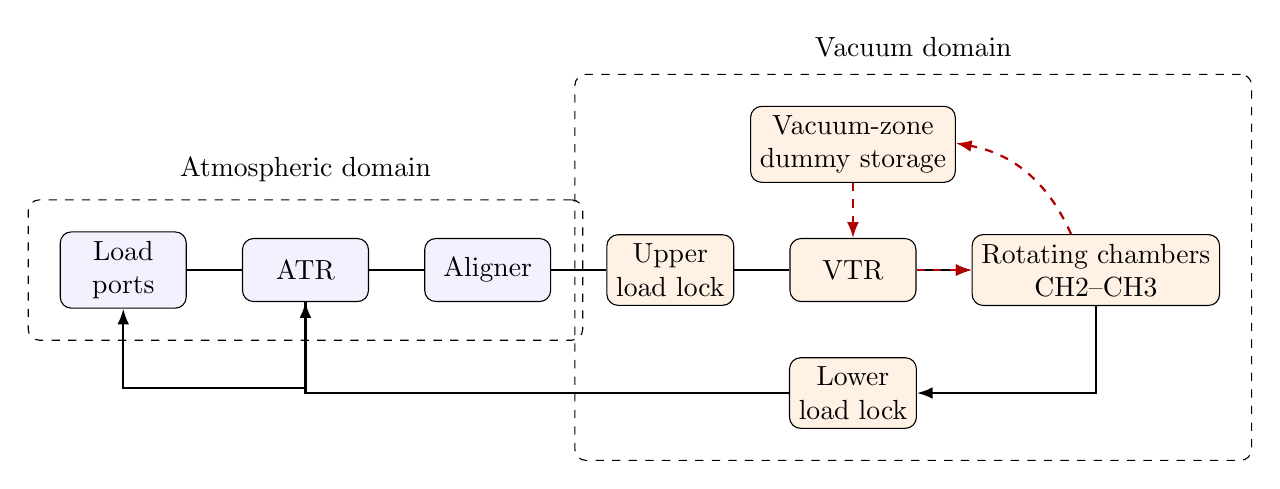
\begin{tikzpicture}[
node distance=7mm and 7mm,
box/.style={draw,rounded corners,align=center,minimum height=8mm,minimum width=16mm,fill=blue!5},
vbox/.style={box,fill=orange!10},
flow/.style={-{Latex[length=2mm]},thick},
dflow/.style={-{Latex[length=2mm]},thick,dashed,red!70!black},
domainbox/.style={draw,dashed,rounded corners,inner sep=4mm}]
\node[box] (lp) {Load\\ports};
\node[box,right=of lp] (atr) {ATR};
\node[box,right=of atr] (al) {Aligner};
\node[vbox,right=of al] (llu) {Upper\\load lock};
\node[vbox,right=of llu] (vtr) {VTR};
\node[vbox,right=of vtr,minimum width=27mm] (ch) {Rotating chambers\\CH2--CH3};
\node[vbox,below=of vtr] (lll) {Lower\\load lock};
\node[vbox,above=of vtr] (store) {Vacuum-zone\\dummy storage};
\draw[flow] (lp)--(atr)--(al)--(llu)--(vtr)--(ch);
\draw[flow] (ch) |- (lll);
\draw[flow] (lll) -| (atr);
\draw[flow] (atr) -- ++(0,-15mm) -| (lp);
\draw[dflow] (store)--(vtr);
\draw[dflow] (vtr)--(ch);
\draw[dflow] (ch) to[bend right=28] (store);
\node[domainbox,fit=(lp)(atr)(al)] (atm) {};
\node[domainbox,fit=(llu)(vtr)(ch)(lll)(store)] (vac) {};
\node[above=1mm of atm.north] {Atmospheric domain};
\node[above=1mm of vac.north] {Vacuum domain};
\end{tikzpicture}
}
\caption{Dual-source material flows and shared resources. Solid arrows denote
the product-wafer route; dashed arrows denote reusable vacuum-zone dummy wafers.}
\label{fig:system-new}
\end{figure}

The recipe determines how the flows interact. In $4\times1$ mode, the chamber
loads a front side, rotates, loads a back side, processes both sides, and
unloads them in reverse order. A product-deficient final side is completed by
dummy wafers. In $2\times2$ mode, product pairs form a chain: adjacent
exposures share an intermediate pair, while leading and trailing positions
require dummy pairs. Cleaning interrupts the chain only at a legal exposure
boundary and uses a dummy-only chamber cycle. A physical dummy wafer cannot be
assigned to overlapping chamber occupancies.

This interaction creates three decision layers. The \emph{material layer}
chooses recipe groups, chambers, sides, cleaning epochs, and physical dummy
wafers. The \emph{resource layer} orders all operations competing for robots,
load locks, and chambers. The \emph{timing layer} assigns event times and
enforces residence limits. These layers must be optimized jointly because a
material choice changes both the resource conflicts and the feasible timing
network.

\subsection{Decision structure and principal constraints}

Let $\mathcal W$ denote product wafers, $\mathcal C$ the rotary chambers,
$\mathcal O$ the operations, and $\mathcal R$ the unit-capacity resources.
Binary variables $x$ assign product pairs to recipe positions, $u$ activate
batches and chain positions, $a$ assign process cycles to cleaning epochs,
$g$ assign dummy operations to physical dummy wafers, and $y$ order operations
that share a resource. Each operation $o$ has start $s_o$, completion
$e_o=s_o+d_o$, and fixed duration $d_o$.

The central model relations are compactly represented by
\begin{align}
&\sum_{k\in\mathcal K(p)}x_{pk}=1 && p\in\mathcal P, \label{eq:new-assign}\\
&x_{pk}\le u_k,\qquad u_{k+1}\le u_k, && k\in\mathcal K, \label{eq:new-activate}\\
&s_{o'}\ge e_o+\delta_{oo'}, &&(o,o')\in\mathcal A, \label{eq:new-prec}\\
&s_{o'}\ge e_o+\rho^r_{oo'}-M(1-y^r_{oo'}), &&o,o'\in\mathcal O_r,\label{eq:new-res1}\\
&s_o\ge e_{o'}+\rho^r_{o'o}-My^r_{oo'}, &&o,o'\in\mathcal O_r,\label{eq:new-res2}\\
&\sum_{\tau\in\mathcal T_c}g_{j\tau}=1 &&j\in\mathcal J_c^{\rm DW}.\label{eq:new-dummy}
\end{align}
Equation~\eqref{eq:new-assign} makes every product group part of exactly one
recipe position. Equation~\eqref{eq:new-activate} links assignments to a
contiguous active structure. Technological arcs in
Eq.~\eqref{eq:new-prec} create complete product and dummy routes. The paired
disjunctions~\eqref{eq:new-res1}--\eqref{eq:new-res2} prevent overlap on the
ATR, aligner, load-lock slots, VTR, chambers, and each reusable dummy wafer;
the setup term $\rho$ includes endpoint-dependent robot repositioning.

Table~\ref{tab:rule-map-new} connects the remaining industrial rules to their
mathematical role. This mapping is important because feasibility is a property
of the complete equipment trajectory, not only of chamber occupancy.

\begin{table}[htbp]
\centering
\caption{Industrial rules represented by the MILP.}
\label{tab:rule-map-new}
\begin{tabular}{p{0.25\linewidth}p{0.33\linewidth}p{0.32\linewidth}}
\toprule
Industrial rule & Mathematical mechanism & Scheduling consequence \\
\midrule
Rotary side sequence & Event equalities and precedence arcs & Enforces load--rotate--process--unload physics \\
Mixed $4\times1$/$2\times2$ recipes & Assignment, activation, and adjacency links & Selects feasible grouping and shared exposures \\
Cleaning interval & Cycle-to-epoch assignment and capacity & Inserts dummy-only cleaning at legal boundaries \\
Reusable dummy inventory & Physical-wafer assignment plus interval disjunction & Prevents simultaneous reuse of one dummy wafer \\
Robot/load-lock capacity & Endpoint-dependent resource ordering & Prevents transfer conflicts and includes repositioning \\
Residence restrictions & Upper bounds between paired route events & Protects time-sensitive products and transfers \\
Finite-batch throughput & Latest return-to-load-port variable & Measures end-to-end rather than chamber-only completion \\
\bottomrule
\end{tabular}
\end{table}

Cleaning epochs satisfy
\begin{equation}
\sum_v a_{vce}\le H z_{ce},
\end{equation}
where $H$ is the maximum number of process cycles between cleans and $z_{ce}$
activates epoch $e$. Linking constraints insert a dummy-only clean between
consecutive epochs and allow a $2\times2$ chain to split only at an exposure
boundary. Residence limits take the form
\begin{equation}
0\le s_{\mathrm{out}(w,r)}-e_{\mathrm{in}(w,r)}\le \overline R_{wr}.
\end{equation}

\subsection{Throughput first, schedule quality second}

Stage one minimizes the return time of the last product wafer:
\begin{equation}
\cmax\ge e_w^{\rm return}\quad(w\in\mathcal W),\qquad
\min_{z\in\mathcal F}\cmax(z),
\label{eq:new-stage1}
\end{equation}
where $\mathcal F$ contains all material, rotary, cleaning, resource, and
timing constraints. A makespan objective alone is insufficient operationally.
Once the last return time is fixed, many schedules may be equivalent in
$\cmax$ but differ substantially in intermediate product waiting, extreme
holds, and chamber cadence. Those differences affect exposure consistency,
work-in-process residence, and recovery from small disturbances.

Let $\widehat z$ be the best stage-one schedule and $\widehat C$ its makespan.
Stage two retains its discrete material and resource structure
$\mathcal D_{\rm fix}$ and imposes
\begin{equation}
z_d=\widehat z_d\ (d\in\mathcal D_{\rm fix}),\qquad
\cmax(z)\le \widehat C+\varepsilon_C.
\label{eq:new-fix}
\end{equation}
It then minimizes
\begin{equation}
\Phi(z)=\lambda_1 Q_{\rm total}+\lambda_2 Q_{\max}
+\lambda_3 D_{\rm cadence}+\lambda_4 E_{\rm cap},
\label{eq:new-stage2}
\end{equation}
where $Q_{\rm total}$ and $Q_{\max}$ capture avoidable route waiting,
$D_{\rm cadence}$ measures deviations between consecutive chamber starts,
and $E_{\rm cap}$ penalizes soft wait-cap excess.

Equation~\eqref{eq:new-fix} gives the two-stage model a clear guarantee. The
second stage cannot worsen the retained makespan and cannot change the chosen
recipe, assignment, cleaning, or resource-order structure. If stage one proves
optimality, the refined schedule remains globally makespan-optimal; its timing
is optimal for Eq.~\eqref{eq:new-stage2} within the retained discrete
structure. If stage one ends with an incumbent, the same statement holds
relative to that incumbent. The model therefore separates objectives without
disconnecting them from the same physical schedule.

\subsection{Modeling advance}

The formulation extends existing rotating or multi-space models in four
directions simultaneously: finite rather than steady-state scheduling; two
material sources rather than one; endogenous mixed-recipe grouping rather
than a fixed sequence; and conditional schedule-quality refinement rather
than makespan alone. This combination matters because dummy availability,
cleaning, and rotary-side decisions alter the robot conflict graph itself.
They cannot be appended as independent capacity constraints after a product
sequence has been selected.

The same structure explains computational difficulty. Assignment, activation,
epoch, dummy identity, and pairwise order binaries interact with a dense event
time network. The resulting cuts may affect different physical roles even
when their generic efficacy scores are similar. This observation motivates
the solver design in the next section.

\section{Structure-aware learning-enhanced exact solution}
\label{sec:method-new}

\subsection{From model structure to solver guidance}

The MILP exhibits two practical symptoms: finding the first competitive
incumbent can be slow, and generic cut scores do not reveal whether a cut
tightens discrete equipment choices, continuous timing, or their coupling.
\method{} addresses the symptoms at complementary points. SPBS supplies
primal guidance before branch-and-cut, while the learned selector supplies
dual guidance during separation. Both components remain advisory: SCIP keeps
the original feasible region, validates incumbents, generates valid cuts, and
retains proof responsibility.

\subsection{Structure-preserving binary-skeleton warm start}

SPBS extracts the high-confidence binary skeleton of a schedule: product
assignment, batch activation, cleaning epoch, load-lock placement, and safe
local order decisions. Continuous event times and globally sensitive VTR
orders remain free. A temporary MIP completes this partial skeleton and returns
a physically feasible schedule. Only that schedule---not the temporary fixing
constraints---is injected into the original model.

This design is stronger than an arbitrary primal hint. The retained decisions
encode the combinatorial architecture that the detailed timing model must
otherwise discover from scratch, while the completion solve repairs local
timing interactions. Because the original model receives only a feasible
incumbent, SPBS cannot remove a better solution or weaken an optimality proof.

\subsection{Variable-role reconstruction and hierarchical decoding}

HEM describes candidate cuts with 13 generic statistics. We add ten structural
features derived from solver metadata. Variables are partitioned into binary,
general integer, objective-active continuous, auxiliary continuous, and other
roles. For cut $i$, the coefficient mass on role $g$ is
\begin{equation}
p_{ig}=\frac{\sum_{j:x_j\in g}|a_{ij}|}
{\sum_j|a_{ij}|+\varepsilon}.
\label{eq:new-role}
\end{equation}
Role masses, bounded-variable mass, coefficient sign balance,
discrete--continuous coupling, dominant-role mass, and role entropy extend the
representation to 23 dimensions. The features are invariant to variable names
but distinguish the physical function of a cut.

A high-level policy selects the cut budget and a low-level pointer policy
orders candidates. Independent SCIP trajectories are sampled in parallel and
optimized with an A3C-inspired policy-gradient scheme whose reward is negative
PDI. At inference, bounded beam search keeps alternative partial sequences
instead of committing to the first locally best cut. Role-submodular
completion then adds candidates that balance policy score, immediate cut
quality, role coverage, and representation of the remaining pool. The
mechanisms are complementary: reconstruction supplies meaningful diversity;
beam decoding explores alternative orders; completion prevents the final set
from collapsing onto one variable role.

\subsection{Exactness and computational scope}

\method{} ranks only cuts already generated and certified as valid by SCIP.
SPBS adds only a solver-checked incumbent. Consequently, neither component
changes the objective, constraints, integrality requirements, or lower-bound
logic. The method can improve anytime behavior while preserving the same
mathematical meaning of feasibility and optimality as default SCIP. The
supplementary material documents the reproducibility protocol.

\section{Computational results and analysis}
\label{sec:results-new}

\subsection{Evidence structure}

The study uses six complementary evidence sets. Four exact cases verify the
physical formulation. A 2700-run nominal matrix compares seven methods over
20 manufacturing instances and independent solver and training realizations.
A 960-run matched experiment isolates SPBS. A 1500-run control isolates the
second-stage mechanism and its objective. A 300-run factorial design explains
how wafer count, recipe composition, and process scale shape difficulty. An
80-run one-factor study tests operational solvability under parameter
perturbations. All saved incumbents supporting reported conclusions pass
independent checks of the corresponding physical MIP.

PDI is the primary anytime metric because it measures the quality of the
entire primal--dual trajectory; lower is better. Repetitions are aggregated
within manufacturing instances before paired bootstrap intervals, Wilcoxon
tests, and Holm adjustment are calculated. This prevents repeated random seeds
from being treated as independent manufacturing evidence
\citep{gleixner2021miplib}. Hardware, budgets, hyperparameters, complete
matrix definitions, and validation tolerances are reported in the supplement.

\subsection{The formulation represents the intended equipment}

Table~\ref{tab:new-validation} reports four exact pure and mixed-flow cases.
Both stages reach zero gap, and independent reconstruction confirms every
route, resource, cleaning, residence, and dummy-allocation constraint.

\begin{table}[htbp]
\centering
\caption{Exact verification of the two-stage formulation.}
\label{tab:new-validation}
\resizebox{\linewidth}{!}{%
\begin{tabular}{lrrrrr}
\toprule
Configuration & Products & $\cmax$ & Route-total wait & Route-maximum wait & Time (s) \\
\midrule
Pure $4\times1$ & 4  & 458 & 380 & 76 & 0.009 \\
Pure $2\times2$ & 4  & 584 & 112 & 28 & 0.039 \\
Mixed flow & 8  & 834 & 506 & 76 & 0.458 \\
Mixed flow & 16 & 1170 & 1550 & 99 & 24.390 \\
\bottomrule
\end{tabular}
}
\end{table}

The verification does more than show that the code runs. Pure cases recover
the distinct rotary logic of each recipe, while mixed cases require both
recipe structures, two load-lock paths, shared robots, and dummy reuse to
coexist in one feasible trajectory. The rapid growth in search effort from
the small pure cases to the 16-product mixed case confirms that the difficulty
comes from coupled assignment and resource order, precisely the structure
targeted by \method{}.

\subsection{\method{} provides the strongest mean anytime performance}

Table~\ref{tab:new-main} gives the full nominal comparison. \method{} has the
lowest mean PDI and the shortest mean solution time among all seven methods.
Its mean PDI is 1.41\% below adapted HEM and 1.97\% below default SCIP. Every
one of its 500 runs returns a feasible incumbent.

\begin{table}[htbp]
\centering
\caption{Nominal comparison; statistics are first averaged within 20 manufacturing instances.}
\label{tab:new-main}
\resizebox{\linewidth}{!}{%
\begin{tabular}{lrrrr}
\toprule
Method & Mean PDI & Mean gap (\%) & Mean time (s) & Optimal (\%) \\
\midrule
SCIP & 16919.01 & \textbf{119.54} & 226.05 & \textbf{64.0} \\
Adaptive cut selection & 16854.87 & 127.18 & 222.34 & 62.0 \\
HEM-13D & 16823.18 & 127.24 & 219.65 & 62.4 \\
HEM-13D+Beam & 16829.59 & 127.19 & 219.95 & 62.4 \\
23D Features Only & 16620.91 & 125.33 & 219.42 & 62.6 \\
Structure+Greedy & 16598.11 & 126.03 & 218.44 & 63.2 \\
\method{} & \textbf{16585.70} & 126.01 & \textbf{218.32} & 63.2 \\
\bottomrule
\end{tabular}}
\end{table}

The pattern across methods explains the advantage. Replacing HEM's generic
representation with variable-role features produces the largest component
gain. Adding structural completion improves the mean again, and beam decoding
provides a further improvement only after the representation and completion
mechanism are structure-aware. Beam alone slightly worsens HEM-13D. The result
shows that the benefit does not come from wider decoding in isolation; it
comes from exploring alternatives in a representation that distinguishes the
roles those alternatives play in the scheduling MILP.

SCIP has a marginally better final gap and optimal rate, whereas \method{}
leads PDI and elapsed time. This is an interpretable trade-off rather than a
contradiction. SCIP's default selection remains strong for eventual proof,
while \method{} improves the trajectory by allocating cuts toward the coupled
assignment--timing structure earlier. For time-constrained industrial use,
where an incumbent and its quality during the available horizon matter, the
PDI and time results establish the algorithm's practical advantage.

\subsection{SPBS is the dominant primal mechanism}

The independent SPBS experiment gives the clearest mechanism-level result.
As Table~\ref{tab:new-spbs} shows, automatic SPBS raises incumbent availability
from 51.67\% to 100\% and reduces mean PDI by 26.19\%. The effects remain
significant after Holm adjustment ($p=2.55\times10^{-5}$ and
$p=3.46\times10^{-8}$, respectively).

\begin{table}[htbp]
\centering
\caption{Independent SPBS comparison over 48 instances and ten matched seeds.}
\label{tab:new-spbs}
\begin{tabular}{lrrrr}
\toprule
Warm start & Runs & Incumbent (\%) & Optimal (\%) & Mean PDI \\
\midrule
Automatic SPBS & 480 & \textbf{100.00} & 54.58 & \textbf{20278.78} \\
None & 480 & 51.67 & 51.67 & 27473.05 \\
\bottomrule
\end{tabular}
\end{table}

The industrial interpretation is direct. Without a structured start, nearly
half of the runs end before a complete schedule is available. SPBS converts
the equipment's discrete architecture into an incumbent early enough for SCIP
to improve it and use it to prune the tree. The large PDI reduction therefore
reflects both better primal availability and a stronger interaction between
the incumbent and subsequent exact search. SPBS is not merely a convenience
for reporting a feasible schedule; it changes the quality of the entire
anytime trajectory.

\subsection{The second stage creates operationally superior schedules}

Makespan verification alone cannot establish the value of the second stage.
We therefore reconstruct route waits directly from product event times and
cadence directly from active chamber starts. This avoids using objective
slack variables as performance measures and makes the metric identical across
all profiles.

\begin{table}[htbp]
\centering
\caption{Operational effect of conditional schedule refinement.}
\label{tab:new-stability}
\resizebox{\linewidth}{!}{%
\begin{tabular}{lrrrr}
\toprule
Profile & Route-total wait & Route-maximum wait & Cadence CV & Cadence deviation \\
\midrule
Full two-stage model & 2596.01 & 296.33 & \textbf{0.130} & \textbf{22.04} \\
Quadratic refinement & \textbf{2469.47} & \textbf{293.27} & 0.134 & 60.18 \\
No second stage & 5398.60 & 952.57 & 0.216 & 370.41 \\
\bottomrule
\end{tabular}}
\end{table}

Relative to no second stage, the proposed refinement reduces route-total wait
by 51.91\%, maximum route wait by 68.89\%, cadence CV by 39.70\%, and cadence
deviation by 94.05\%; all four effects remain significant after Holm
adjustment. These are large operational changes, not small numerical
preferences between equivalent schedules. Shorter and less extreme waits
reduce residence exposure, while regular chamber starts produce a more stable
rhythm for downstream handling.

The comparison with quadratic refinement adds a second insight. The quadratic
profile has slightly lower route-wait means, but the proposed linear objective
reduces cadence deviation by 63.38\% with a significant matched effect. Thus,
the proposed stage establishes the strongest cadence regularity while retaining
route waits far below the no-refinement schedule. This result confirms its
intended industrial role: remove severe waiting and create a repeatable
processing rhythm without sacrificing throughput.

\subsection{Mixed-flow scale, not uniform processing inflation, drives difficulty}

The factorial results reveal a sharp complexity transition. All 8- and
16-wafer runs prove optimality, but the rate falls to 36\% at 24 wafers and
20\% at 32 wafers. Mean PDI increases from 28.13 and 1876.54 to 31155.94 and
32959.89, respectively.

\begin{table}[htbp]
\centering
\caption{Computational transition by wafer count.}
\label{tab:new-doe}
\begin{tabular}{rrrrr}
\toprule
Wafers & Runs & Optimal (\%) & Mean PDI & Mean time (s) \\
\midrule
8 & 75 & 100 & 28.13 & 0.34 \\
16 & 75 & 100 & 1876.54 & 33.86 \\
24 & 75 & 36 & 31155.94 & 408.55 \\
32 & 75 & 20 & 32959.89 & 433.20 \\
\bottomrule
\end{tabular}
\end{table}

The fitted factorial model ($R^2=0.998$ for PDI) attributes this transition to
the interaction of wafer count and recipe composition. At the $1{:}1$ mix,
the additional PDI interactions are 37729.48 and 40788.63 for 24 and 32 wafers.
By contrast, every prespecified processing-scale main and interaction interval
includes zero. The difficult cases are therefore created by combinatorial
coupling---more products participating in both recipe structures---rather
than by uniformly longer processing durations. This finding supports the
design of \method{}: structural assignment and timing roles are more
informative than a generic measure of problem duration.

\begin{figure}[htbp]
\centering
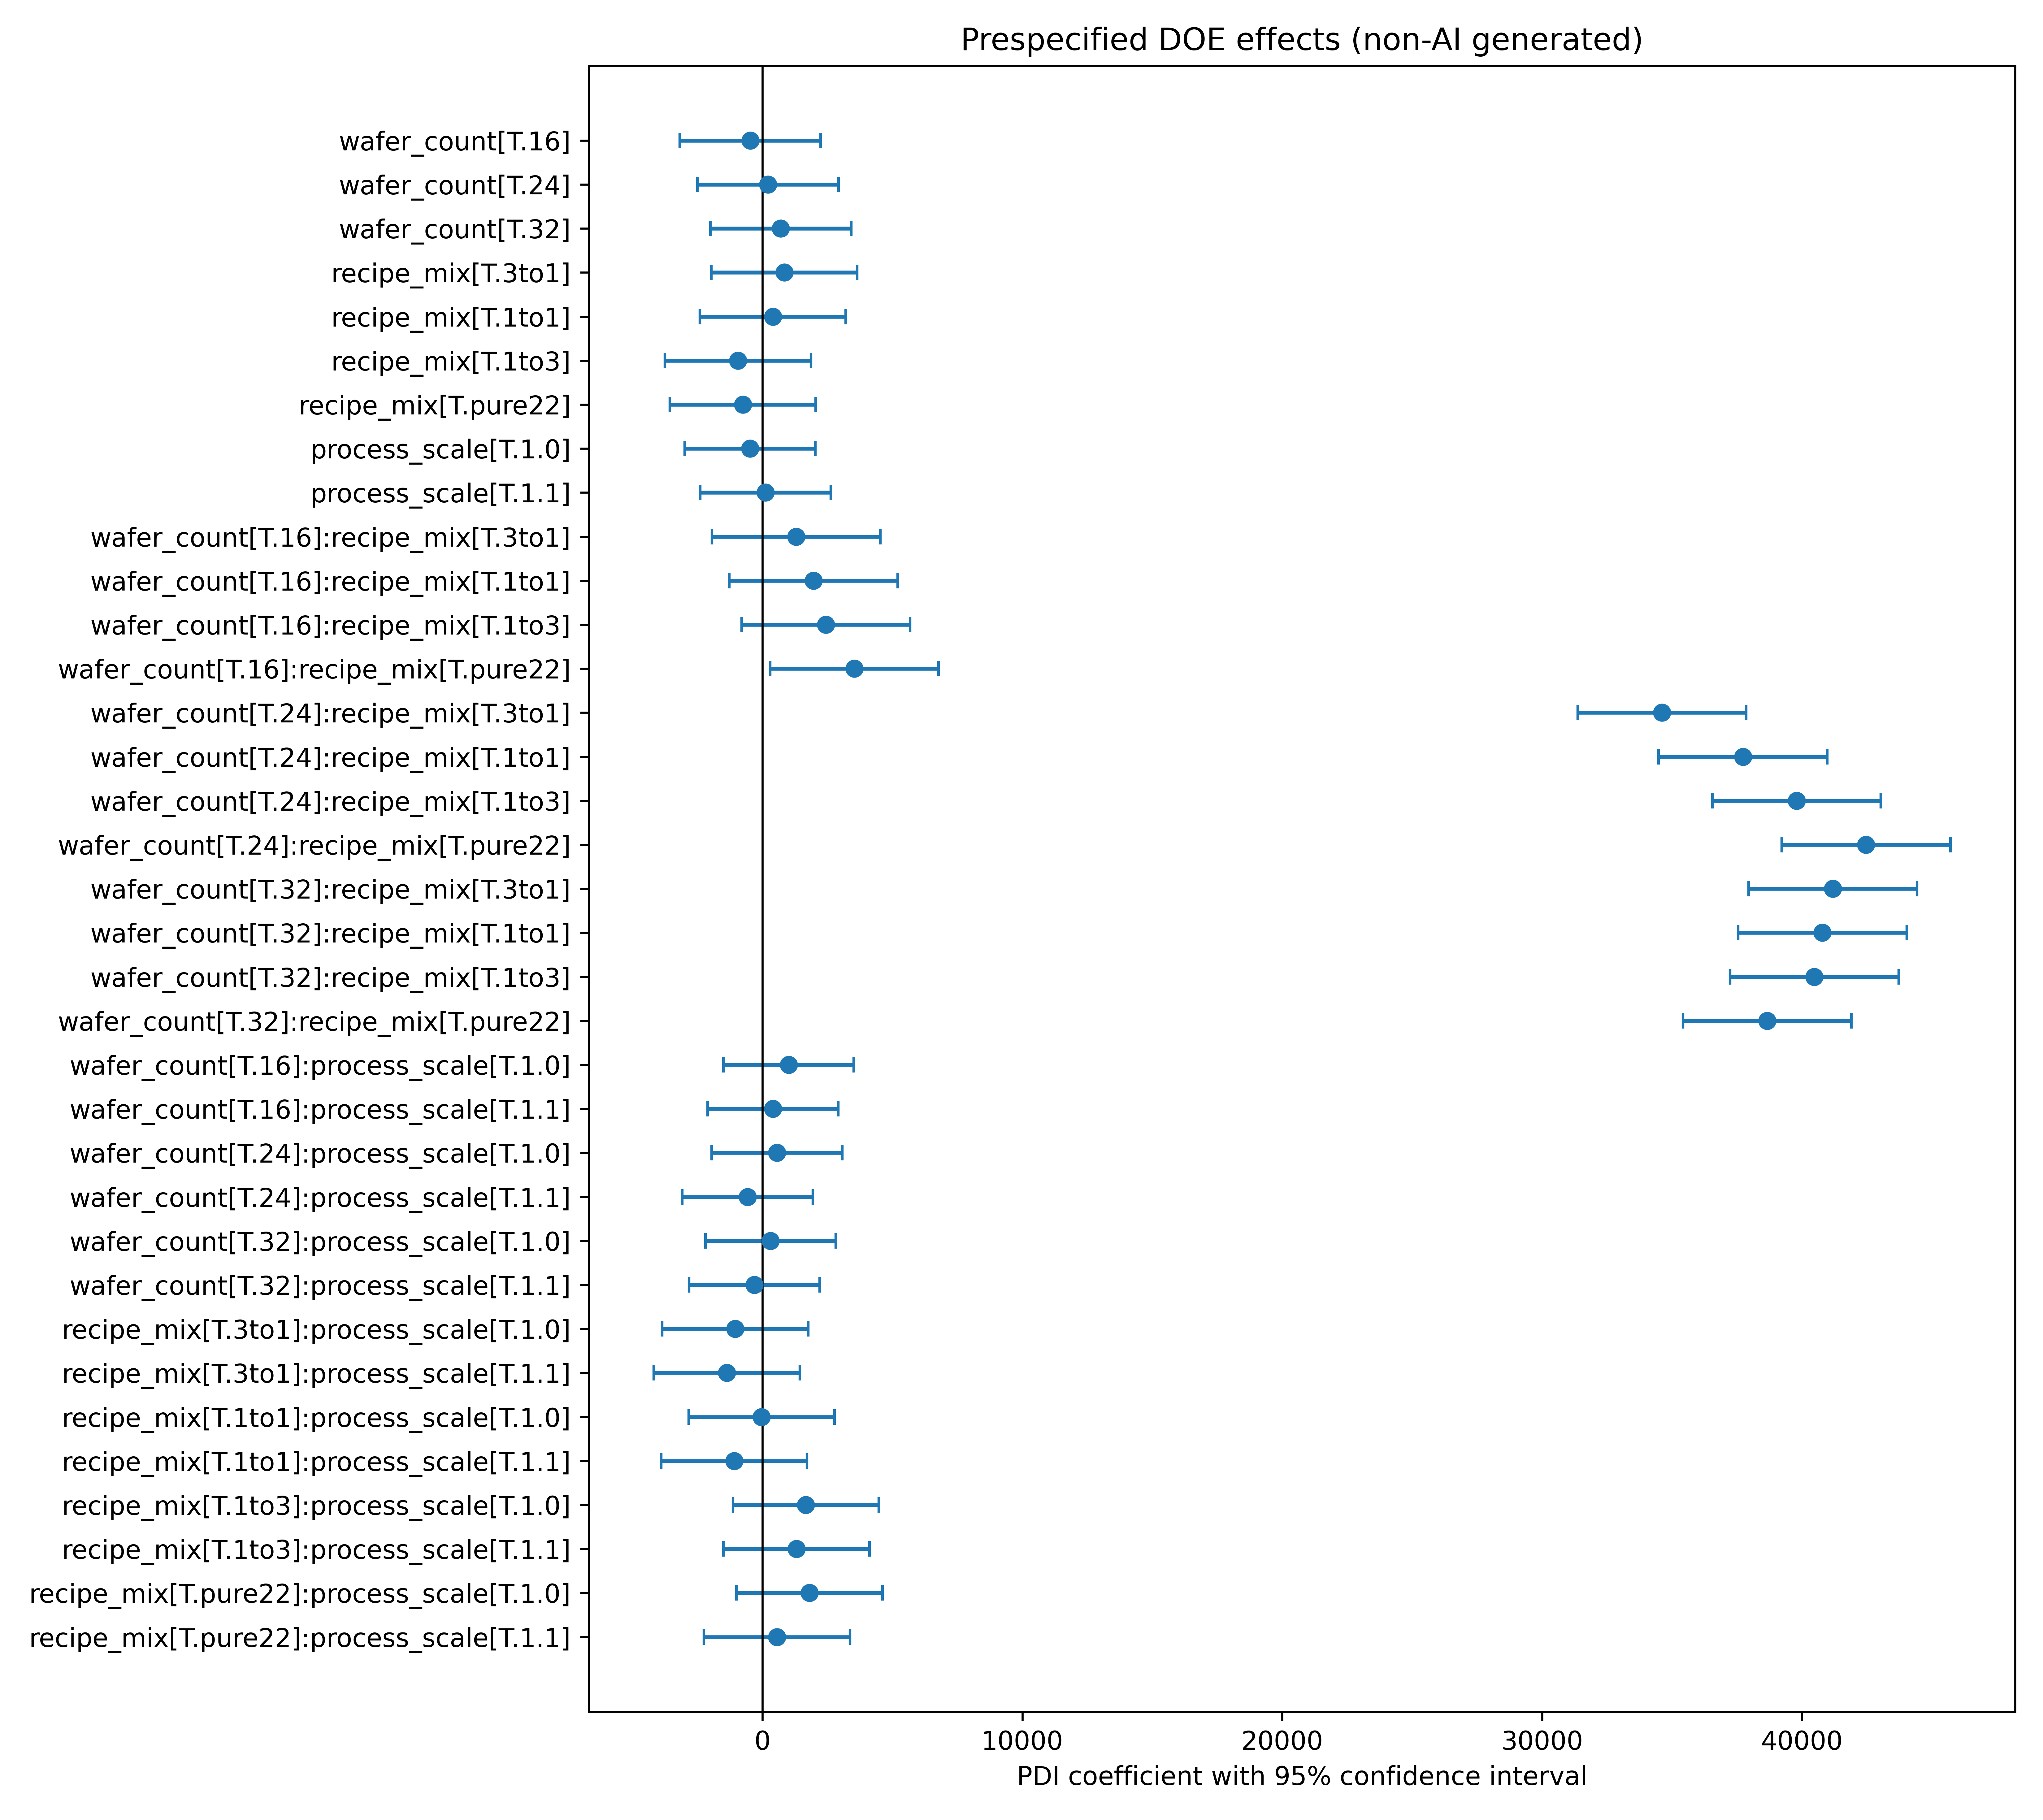
\includegraphics[width=0.96\linewidth]{Figure_DOE_PDI_effects.png}
\caption{Prespecified factorial effects on PDI. Points are OLS coefficients,
bars are 95\% confidence intervals, and the vertical line denotes zero.}
\label{fig:new-doe}
\end{figure}

\subsection{Sensitivity and industrial implications}

All 80 one-factor sensitivity runs return independently valid incumbents.
The lowest mean PDI occurs with a longer cleaning interval (28899.41), whereas
slower motion produces the highest mean PDI (42478.32). The pattern is
physically consistent: less frequent cleaning removes dummy-only interruptions,
while slower transport intensifies conflicts on already shared robots. More
importantly, the formulation and exact-solution chain remain operational
across every prescribed perturbation.

Three implications follow from the complete evidence. First, throughput and
schedule quality should be optimized sequentially: a makespan-only model
leaves substantial avoidable waiting and cadence instability. Second, an
application-feasible incumbent is the most powerful single computational
intervention; SPBS should therefore be treated as part of the solution
architecture rather than a preprocessing detail. Third, learning is most
effective when its representation mirrors the MIP's physical roles. The
observed sign reversal of the beam effect establishes that beam search and
structure-aware representation form a coupled design: beam decoding creates
value after the candidate representation has been aligned with discrete
equipment choices and continuous timing.

The explicit state, resource, and timing layers also provide a direct foundation
for online arrivals, stochastic processing, and module-failure recourse. The
present finite-batch evidence establishes the central result: for dual-source
mixed-flow equipment, the two-stage model produces materially better schedules
and \method{} provides the strongest mean anytime search among the compared
methods.

\section{Conclusions}
\label{sec:conclusion-new}

This paper develops an integrated model-and-algorithm framework for
dual-source mixed-flow rotating-chamber cluster tools. The two-stage MILP
captures the complete interaction of product wafers, reusable vacuum-zone
dummy wafers, mixed rotary recipes, cleaning, shared robots, load locks, and
residence restrictions. Its first stage optimizes end-to-end makespan; its
second stage preserves that production plan and transforms its timing quality.

The experimental results establish the value of both contributions. The full
model yields physically valid pure and mixed schedules, and second-stage
refinement cuts route-total wait, maximum route wait, cadence variation, and
cadence deviation by 51.91\%, 68.89\%, 39.70\%, and 94.05\%. The proposed
\method{} solver records the lowest mean PDI and solution time in the complete
2700-run seven-method comparison. Its SPBS component independently reduces
PDI by 26.19\% and raises incumbent availability to 100\%. Factorial results
further show that the principal difficulty is the interaction between scale
and mixed-recipe composition, exactly the discrete--continuous structure
exposed by the reconstructed features.

The central conclusion is therefore unambiguous: the proposed two-stage MILP
produces operationally superior schedules, and the structure-aware
learning-enhanced branch-and-cut method improves the mean anytime performance
of exact solution. Together they provide a rigorous and practically useful
approach to a class of rotating-chamber scheduling problems that is not
covered by existing single-source or fixed-sequence models.

\section*{CRediT authorship contribution statement}
The authors jointly contributed to conceptualization, methodology, software,
validation, formal analysis, investigation, visualization, and manuscript
preparation.

\section*{Declaration of competing interest}
The authors declare that they have no known competing financial interests or
personal relationships that could have appeared to influence the work
reported in this paper.

\section*{Data and code availability}
The data, mathematical instances, trained models, and source code supporting
the findings are available from the corresponding author on reasonable
request. A permanent public archive will be cited in the version of record.

\section*{Declaration of generative AI and AI-assisted technologies in the writing process}
During the preparation of this work, the authors used OpenAI Codex for
language editing, consistency checking, and code review. The authors reviewed
and edited all AI-assisted output and take full responsibility for the content
of the publication.

\bibliographystyle{elsarticle-harv}
\bibliography{rdmct_cie_references}

\end{document}
